\documentclass[12pt,a4paper,UKenglish]{article}
\usepackage[utf8]{inputenc}
\usepackage[T1]{fontenc, url}
\usepackage{float}
\usepackage{graphicx}
\usepackage{subfig}
\usepackage{babel,csquotes,newcent,textcomp}
\usepackage[backend=biber, sortcites, sorting=none ]{biblatex}
%\usepackage{subfig}
\usepackage{hyperref}
\hypersetup{colorlinks=true, linktoc=none, linkcolor=blue,}
\usepackage [nopostdot, acronym, nogroupskip, nonumberlist,] {glossaries} 
\setacronymstyle{long-short}
\glsdisablehyper

\makenoidxglossaries

\newacronym{ldo}{LDO}{linear dropout}
\newacronym{pcb}{PCB}{printed circuit board}
\newacronym{mos}{MOS}{metal-oxide-semiconductor}
\newacronym{nmos}{nMOS}{n-channel MOS}
\newacronym{pmos}{pMOS}{p-channel MOS}
\newacronym{cmos}{CMOS}{complementary metal-oxide-semiconductor}
\newacronym{vpp}{Vpp}{peak to peak voltage}
\newacronym{vp}{Vp}{peak voltage}
\newacronym{vce}{VCE}{voltage conversion efficiency}
\newacronym{pce}{PCE}{power conversion efficiency}
\newacronym{vtn}{Vtn}{thresold voltage of n-channel MOS}
\newacronym{vtp}{Vtp}{thresold voltage of p-channel MOS}
\newacronym{smps}{SMPS}{switch mode power supply}

\title{Preliminary report on master project}
\author{Rikesh Chauhan}
\date{}

\addbibresource{pre.bib}

\begin{document}
\maketitle

\section{Introduction}
This report is a brief overview of my master project on wireless power transfer through inductive coupling. It is the documentation of the schematic of complete design of the power receiving unit. It includes brief explanation about choices of design topologies and techniques. Figure \ref{fig:blockd} is the block diagram of the complete design including the test \acrshort{pcb} and the test chip on it.

\begin{figure}[htbp] %figure placement: here, top, bottom, or page
   \centering
   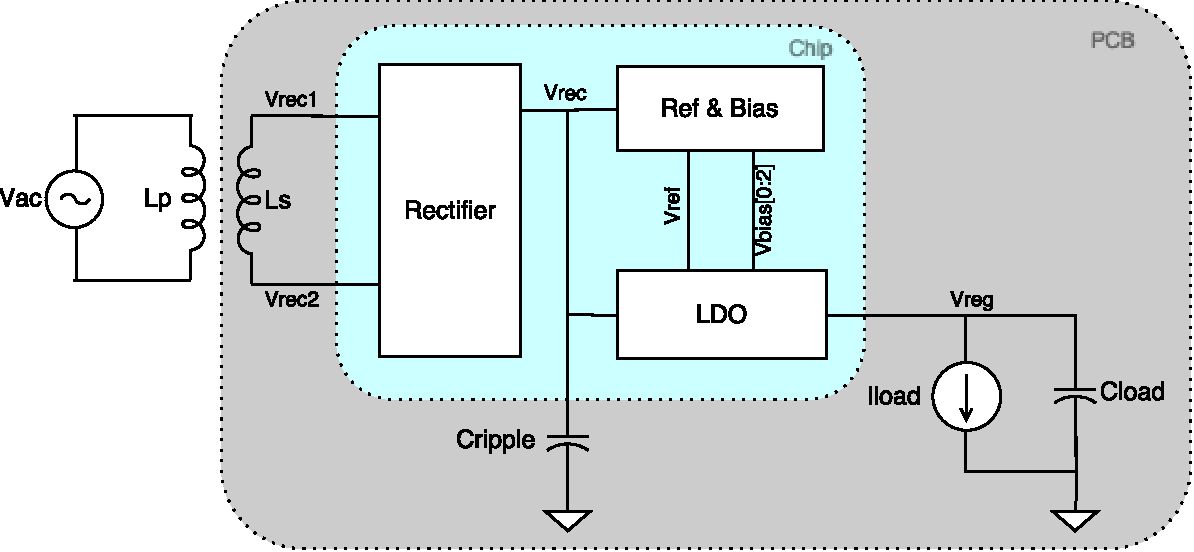
\includegraphics[width=0.8\textwidth]{img/block_diagram.pdf} 
   \caption{Block diagram of complete design}
   \label{fig:blockd}
\end{figure}

As shown in the block diagram above, the design includes inductor, rectifier, \acrshort{ldo} regulator and reference and biasing circuits. This report mainly discusses about the various design aspect of rectifier and \acrshort{ldo}. The inductor is designed with the specifications provided by NORDIC. The biasing and reference circuit is designed solely for learning the design technique without much effort on the accuracy of the generated biases and references. So externally supplied bias and reference will be the secondary option. The project is designed in tsmc90nm process. Table \ref{proj_spec} lists the main specifications of this project.  \\ 

\begin{table}[!htbp]
\caption{Project specifications}
\begin{center}
\begin{tabular}{c|c}
\hline \hline
Technology & TSMC 90nm CMOS \\ \hline
Chip area & TBA mm\textsuperscript{2} \\ \hline
Max. load & 10 mA \\ \hline
Output dc voltage & 1.8 V \\ 
\hline \hline
\end{tabular}
\end{center}
\label{proj_spec}
\end{table}

A brief discussion of the design is followed next.

\newpage

\section{Rectifier}
The most basic rectifier is conventional full wave bridge structure where the diodes are replaced by the diode connected \acrshort{mos}. devices in \acrshort{cmos}. technology. This topology though being simple to implement, has a major drawback. It requires at least twice the $\acrshort{vtn}$ of a MOS device as there are two diode connected MOSes in the conduction path for each cycle of the input signal.  \\

Gate cross coupled and fully gate cross coupled topologies are improvements over conventional full wave rectifier. In gate cross coupled rectifier, two diodes of conventional rectifier is replaced by two gate cross coupled MOSes working as switches where the voltage drop for every cycle is reduced to one threshold voltage. Similarly, in the fully gate cross coupled rectifier, all diodes are replaced by switches and hence the voltage drop is further reduced to twice the conduction drop only for every cycle. Even though this topology has least voltage drop, it suffers from the problem of reverse charge leakage because when the input ac amplitude is less than the output rectified voltage and the conducting pass devices are on simultaneously, current flows backward from output to input. \\

All the above discussed topology suffer from either large voltage drop or large power loss because of which their use are limited in low power and low voltage devices. The popular techniques for higher efficiency are using gate cross coupled rectifier along with passive or active circuitry  for controlling other two pass devices. In passive rectifier, additional circuitry including bootstrap capacitor are used to reduce or eliminate threshold voltage one of which is discussed in this paper \cite{rectboot}. However, use of on-chip bootstrap capacitors limits it use where chip area and speed is of importance. On the other hand, in active rectifier, active circuitry is used control pass devices. The use of active circuitry increase both  \acrshort{vce} and  \acrshort{pce} because the pass devices are made to conduct in linear region and hence less conduction drop, and reverse current flow can be completely eliminated and hence less power loss. However active rectifier is not problem free either. The major issue is starting of the active circuit as there is no regulated supply at the start up. \\

In this project, active rectifier is chosen, primarily for better VCE and PCE and secondarily to avoid the use large on chip capacitors. \cite{rectrcc}  and \cite{rectcomp} have discussed same active rectifier topology with a slight difference in active circuitry. \cite{rectrcc} has implemented comparator with compensating the falling output delay whereas \cite{rectcomp} has implemented comparator with compensating both the falling and the rising output delay in expense of added circuit complexity and power consumption. \cite{rectrcc} has been used here for its simple design. \\

Figure \ref{rect_conv}, \ref{rect_cc} and \ref{rect_rcc} is the CMOS implementation of conventional full wave bridge rectifier, gate cross coupled rectifier and proposed active rectifier in \cite{rectrcc}. The problem with \ref{rect_conv} and \ref{rect_cc} has already been briefly mentioned above. Though  \ref{rect_cc}  is significantly improvement over  \ref{rect_conv} , it is still not a favourable topology with respect to the design technology chosen. In hte gate cross couple rectifier of  \ref{rect_cc}, the cross coupled pMOSes act as switches, so the only voltage drop across them is conduction drop due to channel resistance. However the other two nMOSes are diode connected, so they have at least $Vtn$ drop across them which means $Vac \geq Vdc + Vtn$ for conduction. 

\begin{figure} [htbp]
  \centering 
  \subfloat[Conventional full wave bridge rectifier]  {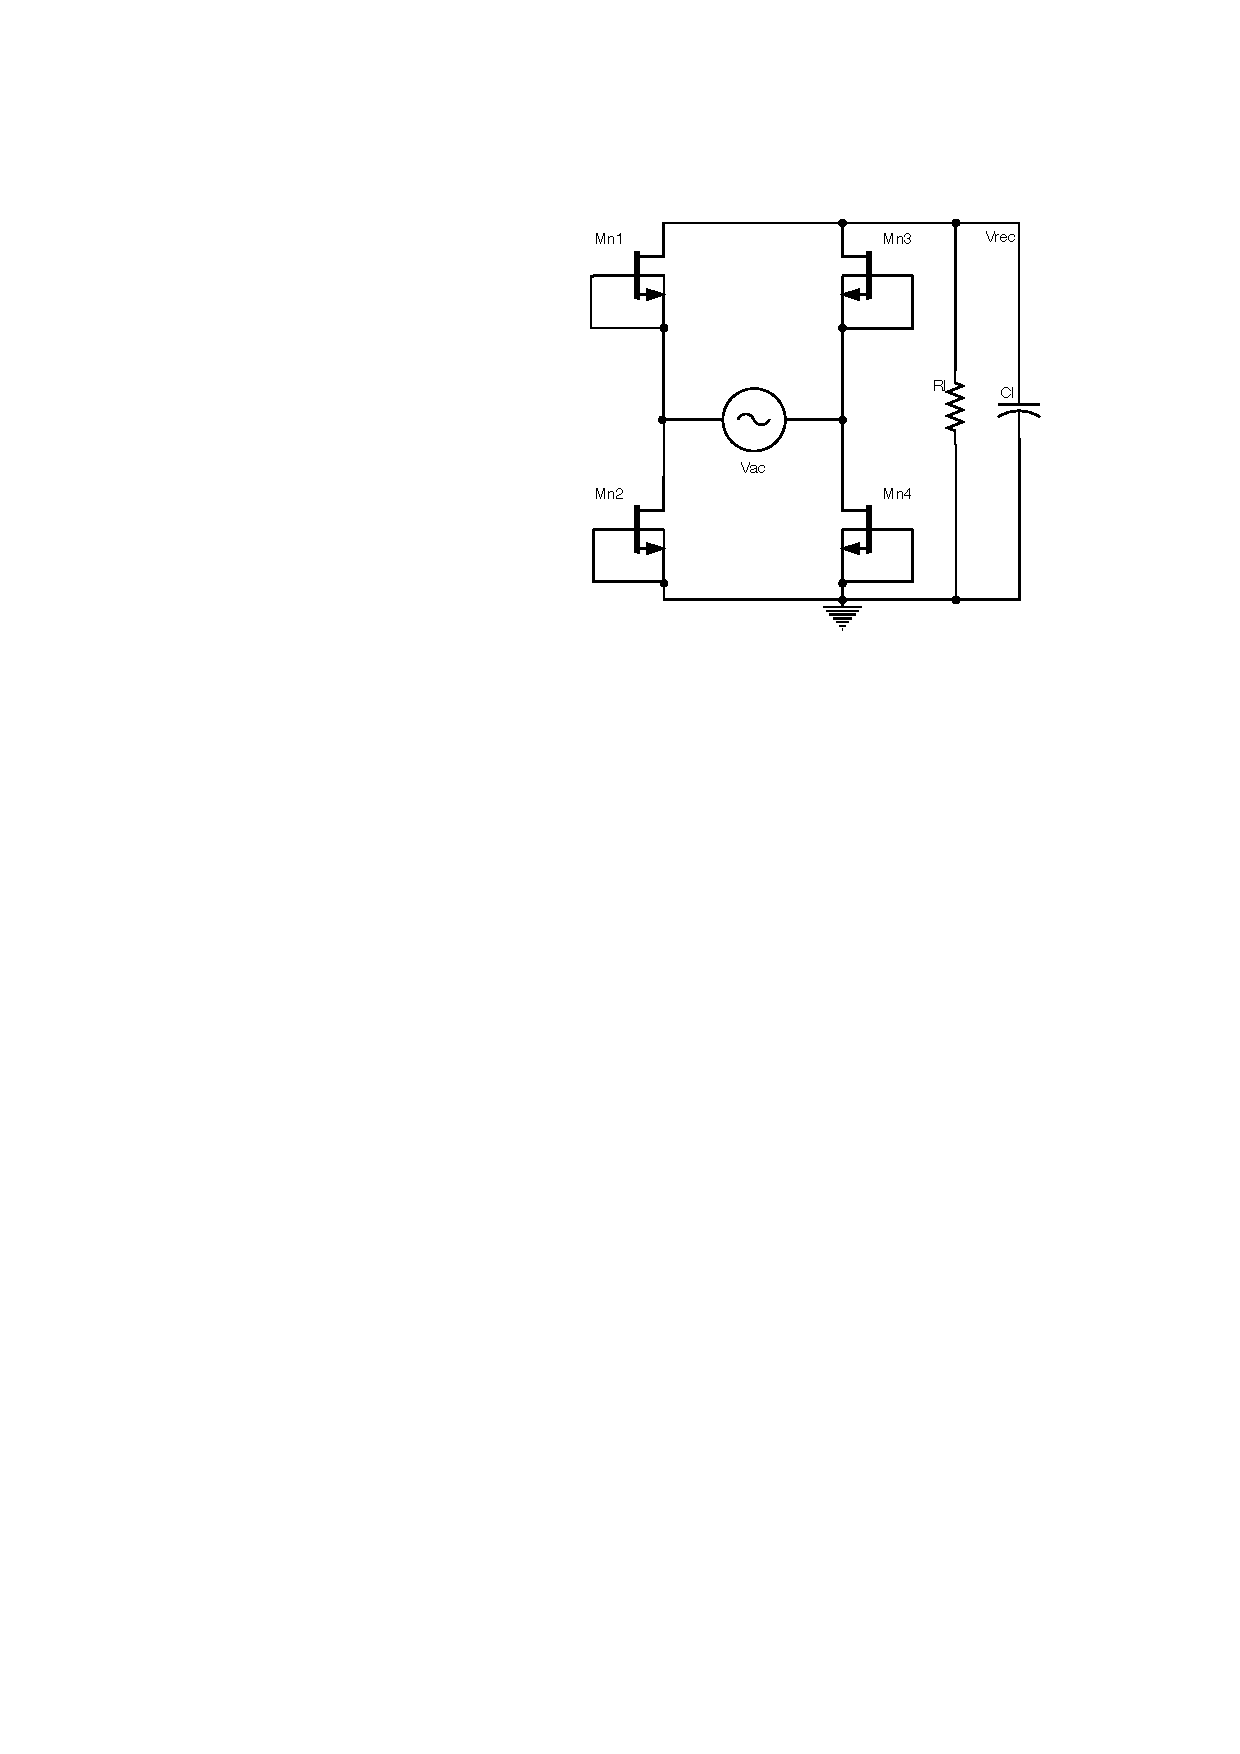
\includegraphics[width=.45\textwidth]{img/rect_conv.pdf} \label{rect_conv}}
\hfill
 \subfloat[Gate cross coupled full wave rectifier]  {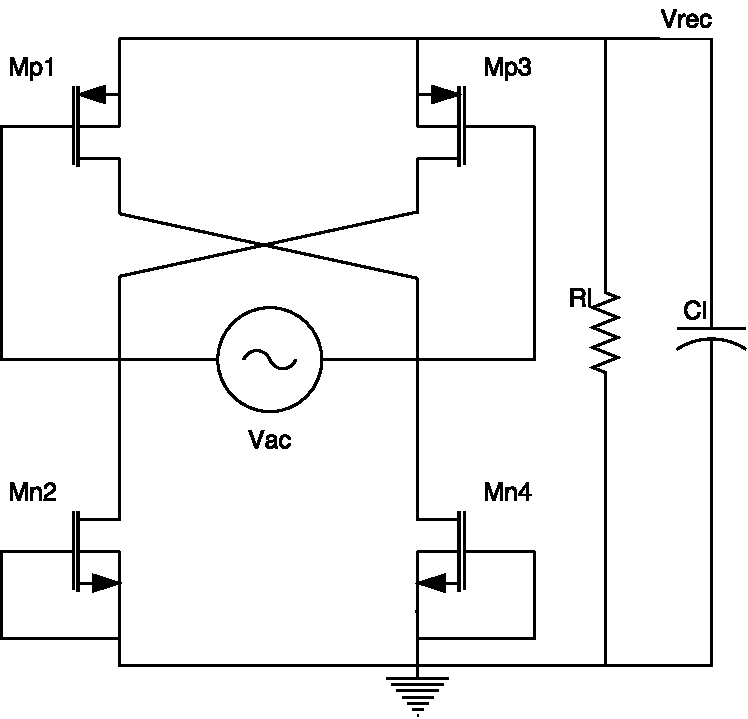
\includegraphics[width=.45\textwidth]{img/rect_cc.pdf}\label{rect_cc}}
 \caption{Rectifier topologies: conventional and gate cross coupled} 
\label{rect_conv_cc} 
\end{figure}

The proposed active circuit in \ref{rect_rcc} is improvement over \ref{rect_cc} which eliminates $Vtn$ drop required for conduction by replacing diode connected nMOS with devices controlled by active circuit as shown in figure \ref{rcc}. The active circuit is a four input comparator that turns on nMOSes fast when Vac > Vdc and turns off fast to avoid flow of current. \\

For the illustration of operation of comparator, consider the case when $Vin1 > Vin2$ i.e. $Vac1 > 0$ and $Vac2 < 0$. During this half cycle, comparator $D1$ and $Mp3$ are reversed biased and hence both are off. For simplicity, assume $Vac =  Vin1 - Vin2$. When $Vac$ reaches $\acrshort{vtp}$, $Mp3$ turns on which shorts $Vin1$ to $Vrec$. When $Vac > Vrec$, $D2$ output goes high, which turns on $Mn4$ and starts the conduction path for the first half cycle and starts charging $Cl$. When $Vac$ reaches maximum, it starts to decrease and at $Vac < Vrec$, conduction stops as output of $D2$ is low and $Mn4$ is off. As $Vac$ further decreases to below $Vtp$, $Mp3$ if off too. This way rectifier in \ref{rect_rcc}  conducts during positive half cycle eliminating the $Vtn$ drop seen in \ref{rect_cc}. Now the only drop is the conduction drop due to channel resistance of two pass devices along the conduction path. This drop is much less because during conduction both the device are operating in the linear region with small resistance. The operation is similar for $Vin2 > Vin1$ where $Mn4$ and $Mp3$ are off and $Mn2$ and $Mp1$ conduct to charge $Cl$. 

\begin{figure} [H]
  \centering 
  \subfloat[Gate cross coupled full wave active rectifer]  {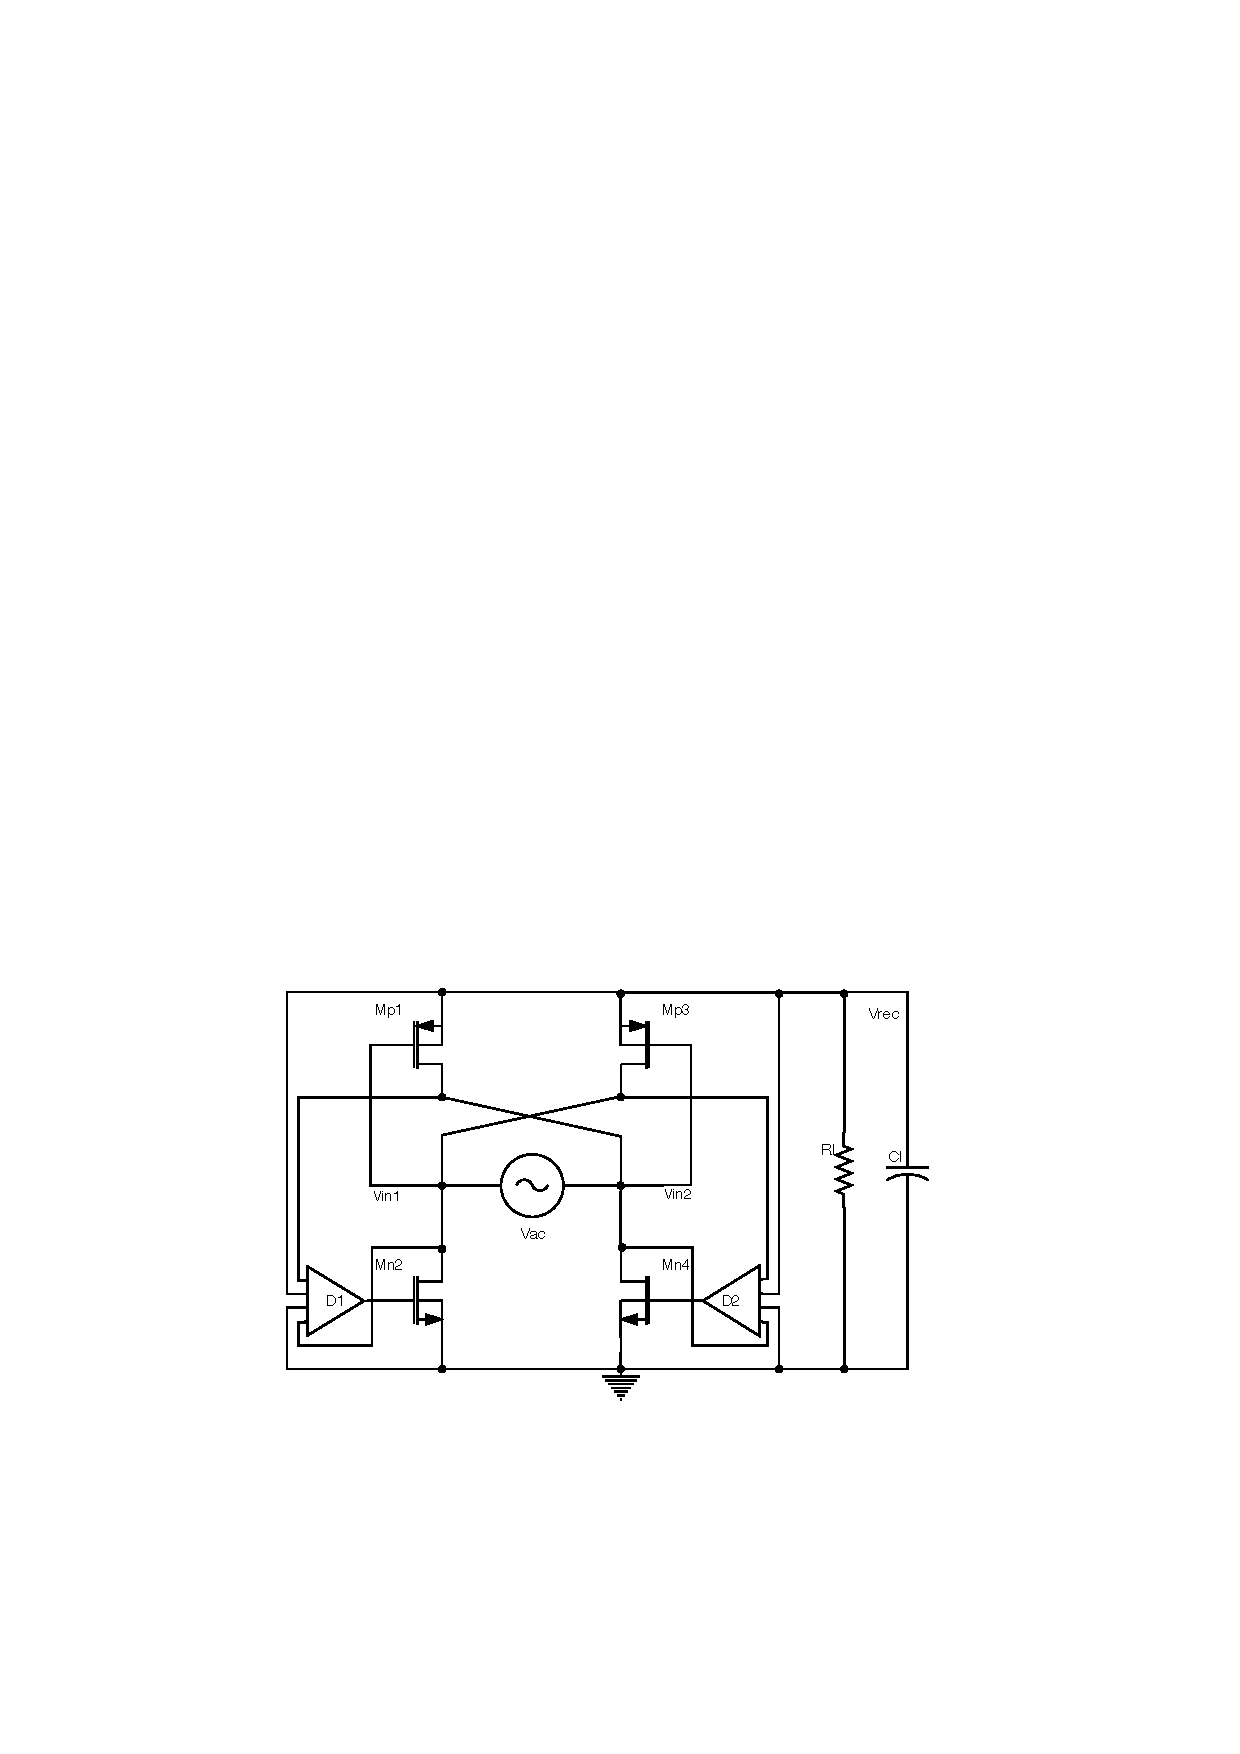
\includegraphics[width=.53\textwidth]{img/rect_rcc.pdf} \label{rect_rcc}}
\hfill
 \subfloat[Active circuit $D2$]  {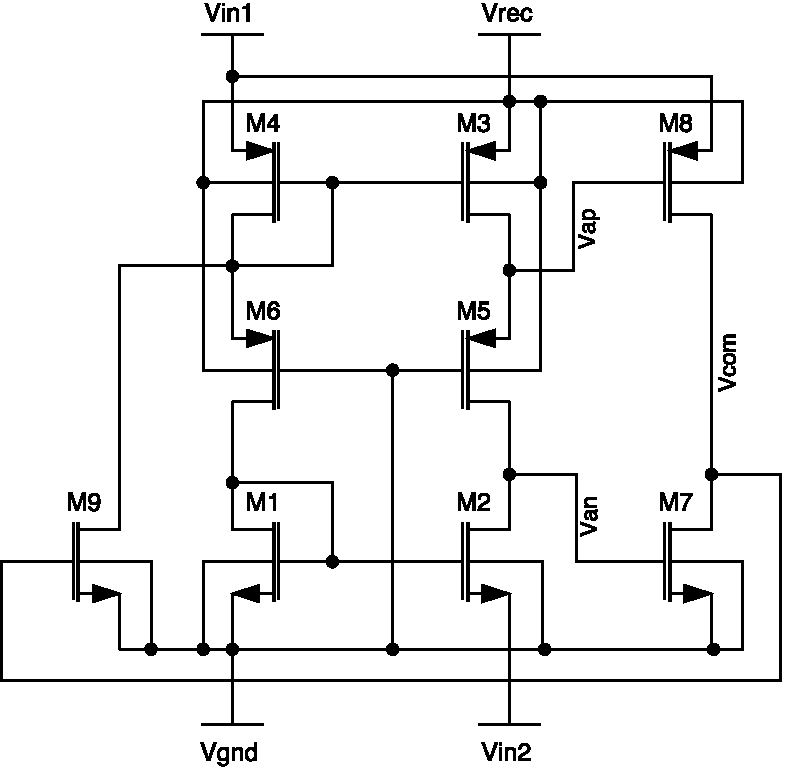
\includegraphics[width=.42\textwidth]{img/rcc.pdf} \label{rcc}}
 \caption{Active rectifier and active circuitry (comparator)} 
\label{rect_rcc_rcc} 
\end{figure}

Figure \ref{rcc}  is the implementation of four input comparator $D2$ used in \ref{rect_rcc} as proposed in \cite{rectrcc}. It is designed to self power and bias because no steady state supply is available at start up. $M1$, $M2$ and $M7$ monitors voltage across $Mn4$ i.e $Vin2 - Vgnd$ and $M3$, $M4$ and $M8$ monitors voltage across $Mp3$ ie $Vin1 - Vrec$ . So when $Vin1 - Vrec > Vin2 - Vgnd$ which means $Vac > Vrec$, output of $D2$ is high and turns on $Mn4$ instantly. But when $Vac < Vrec$, the output of comparator is delayed to fall which causes $Mn4$ to conduct in reverse direction leading to significant reduction in power delivered to load. $M9$ is introduced in order to overcome this problem which adds offset currents to increase $Van$ and $Vpn$ faster, causing the output to decrease faster and turns off $Mn4$ before $Vac < Vrec$. This reverse current control technique compensates the comparator delay and increases the power efficiency of the rectifier. \\

The dimensions of the pass devices are first hand calculated by using square law current equation and devices parameters values given in the technology documents, and later optimised with simulation tool in order to make the rectifier to deliver the required current. Since \acrshort{nmos} does not have to have same device size as \acrshort{pmos} to deliver same current, optimal size ratio equation from \cite{rectsize} is used to find nMOS pass devices sizes.
Similarly, the value of ripple rejection capacitor is chosen 100nF for better ripple rejection at the expense of some additional settling time.

\begin{figure}[htbp] %figure placement: here, top, bottom, or page
   \centering
   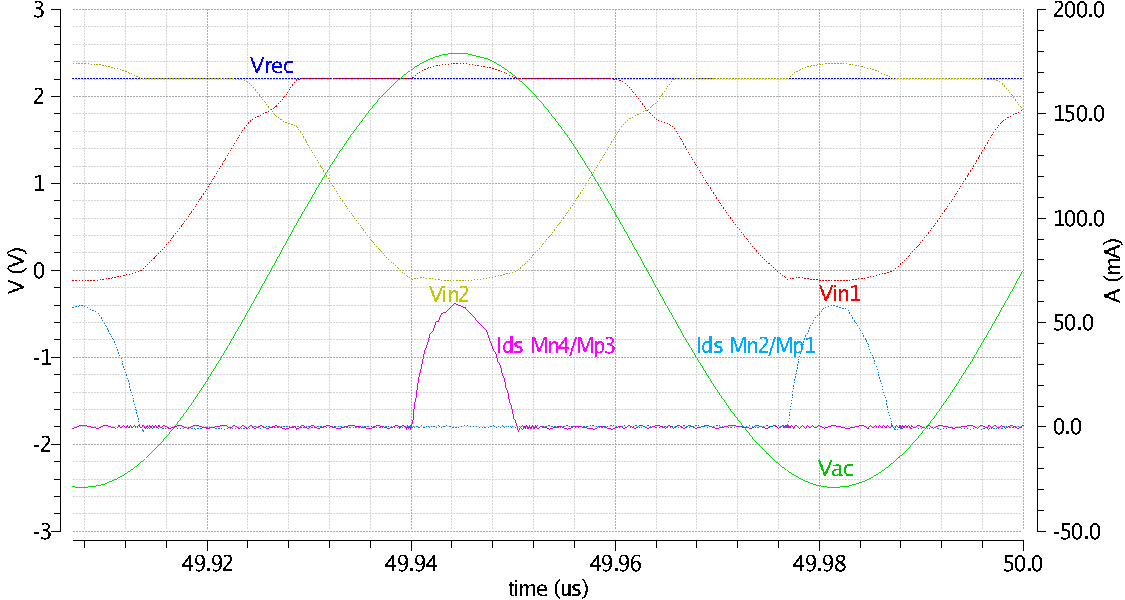
\includegraphics[width=.8\textwidth]{img/rect_output.pdf} 
   \caption{Voltage and current waveforms of the rectifier}
   \label{rect_plot}
\end{figure}

Figure \ref{rect_plot} show the simulation results showing voltages and current waveform of this designed rectifier. The generated waveforms clearly follows the working principle discussed above. Two important observations can be made from plots. First, the rectified output $Vrec$ is 2.2 V for $Vpp$ ac input of 2.5 V which means the voltage loss has been significantly reduced and the loss of around 300 mV yields to the conduction loss due the the channel resistance. Secondly, the reverse current from output to input has been effectively eliminated as there is only positive current flowing to the load when all conducting devices are on.  Similarly, figure  \ref{rect_ce} shows PCE and VCE with respect to magnitude peak ac input signal. Both PCE and VCE are very less for input ac amplitude less then 1.8 V. It can be explained by the fact that required bias current and gate drive voltage are not achieved for smaller input. Finally, table \ref{rect_spec} summarises the rectifier design parameters and its performance.

\begin{figure}[htbp] %figure placement: here, top, bottom, or page
   \centering
   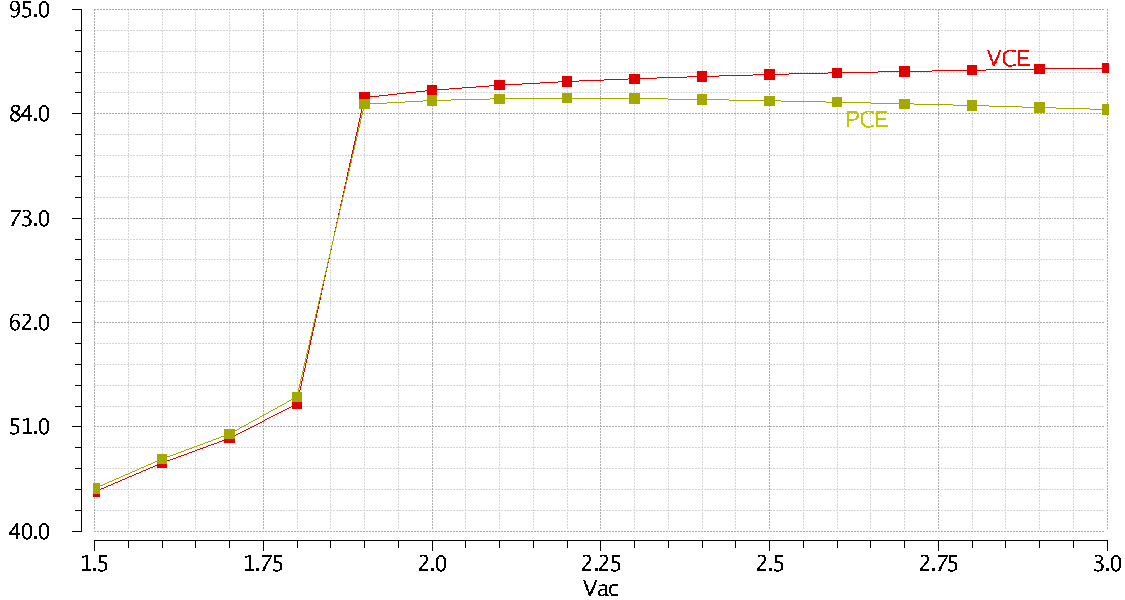
\includegraphics[width=.8\textwidth]{img/rect_ce.pdf} 
   \caption{Voltage and power conversion efficiency}
   \label{rect_ce}
\end{figure}

\begin{table}[htbp]
\caption{Rectifier parameter and performance}
\begin{center}
\begin{tabular}{c|c}
\hline \hline
Wn/Ln, Wp/Lp & 550um/270nm, 900um/270nm \\ \hline
Rectifier area & TBA mm\textsuperscript{2} \\ \hline
Input ac frequency & 13.56 MHz \\ \hline
Input ac \acrshort{vp} & 2.5 V \\ \hline
Load current & 11 mA \\ \hline
Ripple rejection cap & 100nF \\ \hline
Output dc voltage & 2.2 V \\ \hline
Ripple \acrshort{vpp} & 3 mV \\ \hline
PCE & >85\% \\ \hline
VCE & >88\% \\
\hline \hline
\end{tabular}
\end{center}
\label{rect_spec}
\end{table}

LDO design discussion is followed next.

\newpage

\section{LDO}
Voltage regulator follows the rectifier designed above in order to regulated the rectified voltage to 1.8 V and deliver maximum current of 10 mA. Since the output from the active rectifier is 2.2 V and the required regulated voltage is 1.8 V, charge pump or  \acrshort{smps} of boost type is irrelevant here. Buck SMPS could be an option for voltage regulation but LDO is preferred for it better performance in terms of noise. \\

Figure \ref{ldo_gen} shows a circuit of typical pMOS LDO. As shown in the figure, the components includes an error amplifier (EA), a pass device (Mpass), a feedback circuit (R1 and R2) and load (Cout and Iload). A more general and complete LDO circuit also includes the circuitry for generation of reference voltages and bias current/voltages. However, in this project it will be discussed separately for now. In short the working principle of LDO is that the error amplifier compares the scaled down regulated voltage, Vdiv with Vref and regulates the internal resistance of the pass transistor such that  the error, Vref - Vdiv is least or zero ideally. 

\begin{figure}[htbp] %figure placement: here, top, bottom, or page
   \centering
   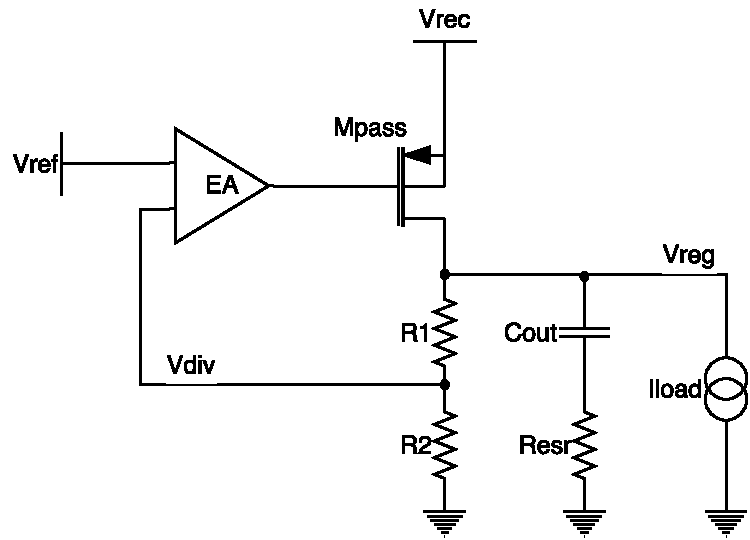
\includegraphics[width=.8\textwidth]{img/ldo.pdf} 
   \caption{LDO with pMOS pass device}
   \label{ldo_gen}
\end{figure}

Figure shows the CMOS implementation of LDO in this project. 

\newpage
\printbibliography

\newpage
\listoffigures

\newpage
\listoftables

%\printindex
\newpage
\printnoidxglossaries

\end{document}
